\documentclass[12pt]{article}
\usepackage[T1]{fontenc}

% Document Details
\newcommand{\CLASS}{AMATH 586}
\newcommand{\assigmentnum}{Numerical SDE Solvers}

\usepackage[margin = 1.1in, top = 1.25in, bottom = 1.in]{geometry}
\usepackage{titling}
\setlength{\droptitle}{-6em}   % This is your set screw
\date{}
\renewcommand{\maketitle}{
	\clearpage
	\begingroup  
	\centering
	\LARGE \sffamily\textbf{\CLASS} \Large \assigmentnum\\[.8em]
	\large Tyler Chen\\[1em]
	\endgroup
	\thispagestyle{empty}
}
 % Title Styling


\usepackage{enumitem}

% Figures
\usepackage{subcaption}

% TikZ and Graphics
\usepackage{tikz, pgfplots}
\pgfplotsset{compat=1.12}
\usetikzlibrary{patterns,arrows}
\usepgfplotslibrary{fillbetween}

\usepackage{pdfpages}
\usepackage{adjustbox}

\usepackage{lscape}
\usepackage{titling}
\usepackage[]{hyperref}


% Header Styling
\usepackage{fancyhdr}
\pagestyle{fancy}
\lhead{\sffamily \CLASS}
\rhead{\sffamily Chen \textbf{\thepage}}
\cfoot{}

% Paragraph Styling
\setlength{\columnsep}{1cm}
\setlength{\parindent}{0pt}
\setlength{\parskip}{5pt}
\renewcommand{\baselinestretch}{1}

% TOC Styling
\usepackage{tocloft}
\iffalse
\renewcommand{\cftsecleader}{\cftdotfill{\cftdotsep}}

\renewcommand\cftchapafterpnum{\vskip6pt}
\renewcommand\cftsecafterpnum{\vskip10pt}
\renewcommand\cftsubsecafterpnum{\vskip6pt}

% Adjust sectional unit title fonts in ToC
\renewcommand{\cftchapfont}{\sffamily}
\renewcommand{\cftsecfont}{\bfseries\sffamily}
\renewcommand{\cftsecnumwidth}{2em}
\renewcommand{\cftsubsecfont}{\sffamily}
\renewcommand{\cfttoctitlefont}{\hfill\bfseries\sffamily\MakeUppercase}
\renewcommand{\cftaftertoctitle}{\hfill}

\renewcommand{\cftchappagefont}{\sffamily}
\renewcommand{\cftsecpagefont}{\bfseries\sffamily}
\renewcommand{\cftsubsecpagefont}{\sffamily}
\fi
 % General Styling
% Code Display Setup
\usepackage{listings,lstautogobble}
\usepackage{lipsum}
\usepackage{courier}
\usepackage{catchfilebetweentags}

\lstset{
	basicstyle=\small\ttfamily,
	breaklines=true, 
	frame = single,
	rangeprefix=,
	rangesuffix=,
	includerangemarker=false,
	autogobble = true
}


\usepackage{algorithmicx}
\usepackage{algpseudocode}

\newcommand{\To}{\textbf{to}~}
\newcommand{\DownTo}{\textbf{downto}~}
\renewcommand{\algorithmicdo}{\hspace{-.2em}\textbf{:}}
 % Code Display Setup
% AMS MATH Styling
\usepackage{amsmath, amssymb}
\newcommand{\qed}{\hfill\(\square\)}

%\newtheorem*{lemma}{Lemma} 
%\newtheorem*{theorem}{Theorem}
%\newtheorem*{definition}{Definition}
%\newtheorem*{prop}{Proposition}
%\renewenvironment{proof}{{\bfseries Proof.}}{}


% mathcal
\newcommand{\cA}{\ensuremath{\mathcal{A}}}
\newcommand{\cB}{\ensuremath{\mathcal{B}}}
\newcommand{\cC}{\ensuremath{\mathcal{C}}}
\newcommand{\cD}{\ensuremath{\mathcal{D}}}
\newcommand{\cE}{\ensuremath{\mathcal{E}}}
\newcommand{\cF}{\ensuremath{\mathcal{F}}}
\newcommand{\cG}{\ensuremath{\mathcal{G}}}
\newcommand{\cH}{\ensuremath{\mathcal{H}}}
\newcommand{\cI}{\ensuremath{\mathcal{I}}}
\newcommand{\cJ}{\ensuremath{\mathcal{J}}}
\newcommand{\cK}{\ensuremath{\mathcal{K}}}
\newcommand{\cL}{\ensuremath{\mathcal{L}}}
\newcommand{\cM}{\ensuremath{\mathcal{M}}}
\newcommand{\cN}{\ensuremath{\mathcal{N}}}
\newcommand{\cO}{\ensuremath{\mathcal{O}}}
\newcommand{\cP}{\ensuremath{\mathcal{P}}}
\newcommand{\cQ}{\ensuremath{\mathcal{Q}}}
\newcommand{\cR}{\ensuremath{\mathcal{R}}}
\newcommand{\cS}{\ensuremath{\mathcal{S}}}
\newcommand{\cT}{\ensuremath{\mathcal{T}}}
\newcommand{\cU}{\ensuremath{\mathcal{U}}}
\newcommand{\cV}{\ensuremath{\mathcal{V}}}
\newcommand{\cW}{\ensuremath{\mathcal{W}}}
\newcommand{\cX}{\ensuremath{\mathcal{X}}}
\newcommand{\cY}{\ensuremath{\mathcal{Y}}}
\newcommand{\cZ}{\ensuremath{\mathcal{Z}}}

% mathbb
\usepackage{bbm}
\newcommand{\bOne}{\ensuremath{\mathbbm{1}}}

\newcommand{\bA}{\ensuremath{\mathbb{A}}}
\newcommand{\bB}{\ensuremath{\mathbb{B}}}
\newcommand{\bC}{\ensuremath{\mathbb{C}}}
\newcommand{\bD}{\ensuremath{\mathbb{D}}}
\newcommand{\bE}{\ensuremath{\mathbb{E}}}
\newcommand{\bF}{\ensuremath{\mathbb{F}}}
\newcommand{\bG}{\ensuremath{\mathbb{G}}}
\newcommand{\bH}{\ensuremath{\mathbb{H}}}
\newcommand{\bI}{\ensuremath{\mathbb{I}}}
\newcommand{\bJ}{\ensuremath{\mathbb{J}}}
\newcommand{\bK}{\ensuremath{\mathbb{K}}}
\newcommand{\bL}{\ensuremath{\mathbb{L}}}
\newcommand{\bM}{\ensuremath{\mathbb{M}}}
\newcommand{\bN}{\ensuremath{\mathbb{N}}}
\newcommand{\bO}{\ensuremath{\mathbb{O}}}
\newcommand{\bP}{\ensuremath{\mathbb{P}}}
\newcommand{\bQ}{\ensuremath{\mathbb{Q}}}
\newcommand{\bR}{\ensuremath{\mathbb{R}}}
\newcommand{\bS}{\ensuremath{\mathbb{S}}}
\newcommand{\bT}{\ensuremath{\mathbb{T}}}
\newcommand{\bU}{\ensuremath{\mathbb{U}}}
\newcommand{\bV}{\ensuremath{\mathbb{V}}}
\newcommand{\bW}{\ensuremath{\mathbb{W}}}
\newcommand{\bX}{\ensuremath{\mathbb{X}}}
\newcommand{\bY}{\ensuremath{\mathbb{Y}}}
\newcommand{\bZ}{\ensuremath{\mathbb{Z}}}

% alternative mathbb
\newcommand{\NN}{\ensuremath{\mathbb{N}}}
\newcommand{\RR}{\ensuremath{\mathbb{R}}}
\newcommand{\CC}{\ensuremath{\mathbb{C}}}
\newcommand{\ZZ}{\ensuremath{\mathbb{Z}}}
\newcommand{\EE}{\ensuremath{\mathbb{E}}}
\newcommand{\PP}{\ensuremath{\mathbb{P}}}
\newcommand{\VV}{\ensuremath{\mathbb{V}}}
\newcommand{\cov}{\ensuremath{\text{Co}\VV}}
% Math Commands

\newcommand{\st}{~\big|~}
\newcommand{\stt}{\text{ st. }}
\newcommand{\ift}{\text{ if }}
\newcommand{\thent}{\text{ then }}
\newcommand{\owt}{\text{ otherwise }}

\newcommand{\norm}[1]{\left\lVert#1\right\rVert}
\newcommand{\snorm}[1]{\lVert#1\rVert}
\newcommand{\ip}[1]{\ensuremath{\left\langle #1 \right\rangle}}
\newcommand{\pp}[3][]{\frac{\partial^{#1}#2}{\partial #3^{#1}}}
\newcommand{\dd}[3][]{\frac{\d^{#1}#2}{\d #3^{#1}}}
\renewcommand{\d}{\ensuremath{\mathrm{d}}}

\newcommand{\indep}{\rotatebox[origin=c]{90}{$\models$}}




 % Math shortcuts


%\usepackage{algorithm}
%\usepackage[noend]{algpseudocode}

\usepackage{amsthm}
\newtheorem*{lemma}{Lemma} 
\newtheorem*{theorem}{Theorem}
\newtheorem*{definition}{Definition}
\newtheorem*{prop}{Proposition}
\renewenvironment{proof}{{\bfseries Proof.}}{\qed}

\hypersetup{
   colorlinks=true,       % false: boxed links; true: colored links
   linkcolor=violet,          % color of internal links (change box color with linkbordercolor)
   citecolor=blue,        % color of links to bibliography
   filecolor=magenta,      % color of file links
   urlcolor=cyan           % color of external links
}


\begin{document}
\maketitle

\section*{Abstract}
This report is intended as a starting reference for numerical methods to SDEs and contains content similar to \cite{holmes,sdes}. The standard text on this topic is \cite{kloeden}, which provides an in-depth approach to stochastic calculus, and numerical methods for SDEs. As a starting point to stochastic calculus in general we refer readers to \cite{lorig}.

\section{Introduction}

A Stochastic Differential Equation (SDE) is an equation of the form,
\begin{align}
    \d X_t =  \mu(X_t,t)\d t + \sigma(X_t,t)\d W_t \label{diffform}
\end{align}
where \( W_t \) denotes a standard Brownian motion \cite{lorig}. We can write this in integral form as,
\begin{align}
    X_{t} - X_{0} = \int_{0}^{t} \mu(s,X_s)\d s + \int_{0}^{t} \sigma(s,X_s) \d W_s \label{intform}
\end{align}

In general we would like to write our solution \( X_T \) as an explicit function of a Brownian motion trajectory. For some processes this is possible, however in general it is not. As a result, numerical methods are required for many SDEs.

SDEs are commonly used to model processes such as molecular dynamics, neurodynamics, financial quantities (stocks, asset prices, interest rates, etc.) SDEs can also be used to efficiently solve high dimensional PDEs numerically, (standard mesh based methods scale exponentially with the dimension of the system).

In this report we first introduce Brownian motion and stochastic calculus. We then discuss how Brownian motion can be approximated numerically and discuss what it means for a numerical SDE method to converge. Next we present simple numerical method and two higher order methods which are obtained using stochastic Taylor expansions. Finally, we conduct some experiments to corroborate the theoretical claims we present earlier in the paper.

\section{Brownian motion}
There are many equivalent characterizations of Brownian motion. Perhaps the most standard is the following definition.
\begin{definition}
A Brownian motion is a stochastic process \( W = (W_t)_{t\geq0} \) defined on some probability space \( (\Omega,\cF,\bP) \) satisfying,
\begin{enumerate}[nolistsep]
    \item \( W_0 = 0 \)
    \item \( (W_d-W_c) \indep (W_b-W_a) \) for all \( 0\leq a\leq b\leq c\leq d \))
    \item \( (W_t - W_s) \sim \cN(0,t-s) \) for all \( 0\leq s\leq t \)
    \item the map \( t \to W_t(\omega) \) is continuous for almost all \( \omega\in\Omega \)
\end{enumerate}
\end{definition}

We attempt to parse this definition and notation. The notation \( W_t \) denotes a random variable which depends on the time \( t \). That is, \( W_t \) is a function from \( \Omega \to \bR \). For a fixed \( \omega \in \Omega \), \( W_t(\omega) \) can be seen as a function of \( t \), and is referred to as a path or a trajectory of the Brownian motion.

Condition 1 means that all paths of the Brownian motion starts start at the origin. Condition 2 means that the random variables \( W_d-W_c \) and \( W_b - W_a \) are independent of one another. That is, knowing how much the a path of the Brownian motion changes over the time interval \( [a,b] \) does not give any information about how much the path changes over the interval \( [c,d] \). Condition 3 means that over any time interval \( [s,t] \) how much the Brownian motion changes is a normal random variable with mean zero and variance \( t-s \). Finally, Condition 4 means that almost all paths of the Brownian motion are continuous.

Brownian motion can be constructed as a scaled random walk. Such a construction can be readily obtained on the internet or in \cite{lorig}. We will simply note that it may be useful to view Brownian motion as the continuous analog to a discrete random walk.

\section{Stochastic Calculus}
In this section we aim to provide enough background to allow all statements in the main portion of the paper to be understood. That said, this done in the admittedly unsatisfying way of black box lemma's and heuristics which we do not explain or prove. For a more complete overview of Stochastic Calculus we refer readers to \cite{kloeden, lorig}.

We first introduce Riemann--Stieltjes integrals.

\begin{definition}
For real valued functions \( f \) and \( g \) the Riemann--Stieltjes integral is defined as,
\begin{align*}
    \int_{a}^{b} f(x) \d g(x) := \lim\limits_{\norm{\Pi}\to 0} \sum_{i=0}^{n-1} f(c_i)(g(x_{i+1}) - g(x_i))
\end{align*}
where \( \Pi = \{a=x_0<x_1 < \cdots < x_n = b\} \) is a partition of \( [a,b] \), \( \norm{\Pi} \) is the length of the largest subinterval, and \( c_i \) is any point in \( [x_i,x_{i+1}] \).
\end{definition}

We note that if \( g(x) = x \) the Riemann--Stieltjes integral is the standard Riemann integral and that if \( g \) is continuously differentiable,
\begin{align*}
    f(g(t)) - f(g(0)) = \int_0^t \d f(g(s)) = \int_0^t f'(g(s))g'(s) \d s
\end{align*}

Brownian motion and many processes involving Brownian motion are not differentiable. It\^o's Lemma gives us a way to compute the analogous result for a class of stochastic processes called It\^o (drift-diffussion) processes. For our purposes we can think of It\^o processes as processes with an integral with respect to \( t \) and an integral with respect to \( W_t \).

\begin{lemma}[It\^o] For \( f:\bR\to\bR \) sufficiently differentiable and It\^o process \( X_t \),
\begin{align}
    \d f(X_t) &=  f'(X_t)\d X_t + \dfrac{1}{2}f''(X_t)\d[X,X]_t %\label{ito}
\end{align}
\end{lemma}
Here we have used the notation \( [X,X]_t \) to denote the quadratic variation of the process \( X_t \). Heuristically we can compute \( \d[X,X]_s \) by expanding  \( (\d X_s)(\d X_s) \) and simplifying using the identities,
\begin{align}
    \d t \d t = 0, && \d t \d W_t = 0, && \d W_t \d W_t = \d t \label{heuristics}
\end{align}


It\^o's Lemma can be generalized to functions and processes of higher dimension.
\begin{lemma}[It\^o] For \( f:\bR^n\to\bR^n \) sufficiently differentiable and It\^o process \( X_t = [X_t^1, X_t^2, \ldots X_t^n]^T \),
\begin{align}
    \d f(X_t) = \sum_{i=1}^{n} \left[\pp{}{x_i}f(X_t)\right] \d X_t^i + \dfrac{1}{2} \sum_{i=1}^{n} \sum_{j=1}^{n}\left[ \pp{}{x_i} \pp{}{x_j} f(X_t) \right] \d [X^i,X^j]_t \label{itond}
\end{align}
\end{lemma}

Similar to before, we compute \( \d[X^i,X^j]_t \) by expanding \( (\d X^i)(\d X^j) \) and using the heuristics in (\ref{heuristics}).

Consider the special case when \( n=2 \), \( X_t^1 = t\), and \( X_t^2 = X_t \). Using our heuristics in (\ref{heuristics}) we have \( \d[X^1,X^2]_t = (\d t)(\d X_t) = 0 \) and \( \d[X^1,X^1] = (\d t)(\d t) = 0 \). Therefore, by (\ref{itond}),
\begin{align}
    \d f(t,X_t) &= \pp{}{t} f(t,X_t) + \pp{}{x} f(t,X_t) \d X_t + \dfrac{1}{2} \pp[2]{}{x}f(t,X_t) \d [X,X]_t
    \\ &= \left( \pp{}{t} + \dfrac{1}{2}\pp[2]{}{x} \right)f(t,X_t)\d t + \pp{}{x} f(t,X_t) \d X_t \label{2dito}
\end{align}


\section{Example Processes}
In this section we provide some results about a few important stochastic processes which we will use in our numerical tests. Both the SDEs we introduce can be solved analytically and the mean and variance can be computed

For constants \( \mu \) and \( \sigma \) a Geometric Brownian motion satisfies,
\begin{align}
    \d X_t = \mu X_t \d t + \sigma X_t \d W_t, && t\in[0,T] \label{GBMeqn}
\end{align}

We will solve this equation to build some familiarity with stochastic calculus.
To this end, note that \( \d X_t = \mu X_t \d t + \sigma X_t \d W_t \) so using the heuristics (\ref{heuristics}) we have \( \d[X,X]_t = \sigma^2 \d t \). We note apply It\^o's Lemma to \( \ln(x) \) to obtain,
\begin{align*}
    \d \ln (X_t) &= \dfrac{1}{X_t} \d X_t - \dfrac{1}{2} \dfrac{1}{X_t^2} \d[X,X]_t
    = \left( \mu - \dfrac{\sigma^2}{2} \right) \d t + \sigma \d W_t
\end{align*}

Integrating both sides from \( T \) to \( t \) we obtain,
\begin{align*}
    \ln (X_t) = \int_0^t \d \ln(X_s) = \int_0^t \left( \mu - \dfrac{\sigma^2}{2} \right)\d s + \int_0^t \sigma \d W_s = \left( \mu - \dfrac{\sigma^2}{2} \right) t + \sigma W_t
\end{align*}

Therefore, the solution to (\ref{GBMeqn}) is,
\begin{align*}
    X_t = X_0 \exp\left( \left( \mu - \dfrac{\sigma^2}{2} \right)t + \sigma W_t \right)
\end{align*}


For constants \( \theta, \mu, \sigma \), an Ornstein--Uhlenbeck (OU) process satisfies,
\begin{align}
    \d X_t = \theta(\mu-X_t) \d t + \sigma \d W_t, && \theta > 0 \label{OUeqn}
\end{align}

We note that if \( X_t \) is away from \( \mu \) it will tend towards this value in expectation. Figure~\ref{OU_em} shows Euler--Maruyama method applied to (\ref{OUeqn}). As expected, the trajectories all end up ``centered'' about \( \mu \). More precisely, (\ref{OUeqn}) has solution,
\begin{align*}
    X_t = X_0 \exp(-\theta t) + \mu(1-\exp(-\theta t)) + \sigma \int_0^t \exp(-\theta(t-s))\d W_s
\end{align*}

The mean of \( X_t \) is,
\begin{align*}
    \bE[X_t] = (X_0 - \mu)\exp \left( -\theta t \right)+ \mu
\end{align*}
Likewise, the variance of \( X_t \) is,
\begin{align*}
    \bE\left[(X_t-\bE[X_t])^2\right] = \dfrac{\sigma^2}{2\theta}(1-\exp(-2\theta t))
\end{align*}

\section{Generating Brownian motion Numerically} \label{brownian_motion}

Given the four properties of Brownian motion, how can we numerically generate trajectories which are representative of a Brownian motion? The most standard way to do this is to first pick a time mesh on which we will have the values of the Brownian motion. Let \( t = [t_0, t_1, \ldots, T] \) where \( 0 = t_0 < t_1 < \cdots < t_N = T \) be such a mesh. We will generate a numerical realization \( \hat{W} = [0, \hat{W}_1, \ldots, \hat{W}_T] \) of a Brownian motion trajectory. To do this we generate the incriments. That is, we start with \( \hat{W}_0 = 0 \) and recursively define,
\begin{align*}
    \hat{W}_{t_{k+1}} = \hat{W}_{t_k} + \Delta \hat{W}_{t_k}
\end{align*}
where, using property (3) of Brownian motion, we must sample \( \Delta \hat{W}_{t_k} \) from a normal distribution with mean 0 and variance \( t_{k+1} -t_{k} \).

Since we only sample at discrete points, we have not generated a ``true'' trajectory of the Brownian motion. In fact, refining the mesh and generating the interior points is not trivial. However, it is clear that the property 2 is satisfied since we sample or increments independently. Similarly, property 3 is satisfied since the sum of iid normal random variables is a iid random variable with mean equal to the sum of the means, and variance equal to the sum of the variances. Therefore this method gives us trajectories which satisfy the first three properties of Brownian motion.

We now make a few practical observations about implementing this procedure on a computer. First, while we have explicitly defined the vector \( \hat{W} \), it may be more efficient to save the vector \( \Delta \hat{W} \) since the numerical methods we present involve \( \Delta W_t \). Second, if it is slow to sample normal random variables, other simpler distributions coud be used. For instance, we could pick \( \Delta W_t \in\{-\sqrt{\d t}, \sqrt{\d t}\} \) with equal probabilities for each choice. In this case the mean and variance will still match Brownian motion, but the higher moments may not (i.e. the increments will no longer be normally distributed). Whether or not this is important is dependent on the application.


\section{Convergence of Numerical Methods}
A SDE solution may have many distinct trajectories as the solution itself is a random process. Our standard definitions of convergence for IVPs are no longer sufficient.

For some applications we would like to be able to compute trajectories numerically which are representative of the actual trajectories of the solution to the SDE. This gives rise to the following definition convergence.
\begin{definition}
A discrete time approximation \( \hat{X}^{(k)} \) is said to converge strongly to the solution \( X_t \) at time \( T \) if,
\begin{align*}
    \lim_{k\to 0}\bE\left[\left| X_T - \hat{X}_T^{(k)} \right|\right] = 0
\end{align*}
and is said to converge strongly with order \( m \) if for sufficiently small \( k \),
\begin{align*}
    \bE\left[\left| X_T - \hat{X}_T^{(k)} \right|\right] = \cO(k^m)
\end{align*}
\end{definition}

Since strong convergence looks at the absolute difference of \( \hat{X}_T^{(k)} \) and \( X_T \) it tells us about how individual trajectories vary. That is, to compute this expectation we first find the absolute difference of our solution and the exact solution for every trajectory of Brownian motion, and then take the mean.

For other applications it may be sufficient to generate trajectories whose moments (mean, variance, etc.) are the same as the trajectories of the solution to the SDE, even if individual trajectories don't necessarily converge to trajectories of the solution. This gives rise to the notion of weak convergence.
\begin{definition}
A discrete time approximation \( \hat{X}^{(k)} \) is said to converge weakly to the solution \( X_t \) at time \( T \) if for every polynomial \( p \),
\begin{align*}
    \lim_{k\to 0} \left| \bE\left[ p(X_T) - p\left(\hat{X}_T^{(k)}\right) \right] \right| = 0
\end{align*}
and is said to converge weakly with order \( m \) if for sufficiently small \( k \) and every polynomial \( p \),
\begin{align*}
    \left|\bE\left[ p(X_T) - p\left(\hat{X}_T^{(k)}\right) \right] \right| = \cO(k^m)
\end{align*}
\end{definition}

Since weak convergence looks at the signed difference of \( \hat{X}_T^{(k)} \) and \( X_T \) the errors can ``cancel'' with one another.


Note that the term corresponding to \( \d t \) is deterministic. This means that if \( \sigma \equiv 0 \), Equation (\ref{intform}) becomes the initial value problem \( \d X_t/\d t = \mu(X_t,t) \) with initial condition at time \( t \) given by the value of \( X_t \). In this case both definitions of convergence agree with the standard definition of convergence for IVPs provided in \cite{leveque}.

We now prove the following (unsurprising) theorem following closely to the proof provided in \cite{holmes}.
\begin{theorem}
The weak order of a SDE method is always less than or equal to the strong order of the method.
\end{theorem}
\begin{proof}
Suppose a method \( \hat{X}^{(k)} \) is strongly convergent. Then the set \( S:=\{\hat{X}_T^{(k)}\}_k\cup\{X_T\} \) is bounded.
Therefore, there exists \( K > 0 \) such that \( K > |p'(x)| \) for all \( x \) in some finite interval containing \( S \).

Since \( |\bE Z| \leq \bE|Z| \) for any random variable \( Z \), and by the Mean Value Theorem,
\begin{align*}
    \left|\bE\left[ p(X_T) - p\left(\hat{X}_T^{(k)}\right) \right] \right|
    \leq \bE\left[\left| p(X_T)  -  p\left(\hat{X}_T^{(k)}\right) \right| \right]
    \leq K \bE\left[\left| X_T - \hat{X}_T^{(k)} \right| \right]
\end{align*}
This proves the result.
\end{proof}

\section{A simple Numerical Method}
All the numerical methods in this report find an approximate solution to a given SDE on some time grid. More specifically, the methods take in a series of time points and the value of a Brownian motion trajectory at these time points and output the approximate solution.

We first introduce the natural generalization of the Forward Euler method. The so called Euler--Maruyama method \cite{sdes} is given by the relation,
\begin{align*}
        \hat{X}_{t+\Delta t} &= \hat{X}_t + \mu(t,\hat{X}_{t}) \Delta t + \sigma(t,\hat{X}_{t}) \Delta W_{t}
\end{align*}
where \( \Delta W_t:=W_{t+\Delta t}-W_t \).


On SDEs where \( \sigma \) and \( \mu \) satisfy the appropriate conditions (these condtions are generally satisifed), the Euler-Maruyama method has strong and weak orders of 1/2 and 1 respectively. A commonly cited proof of this result can be found in \cite{kloeden}. However we note that on some SDEs strong convergence of order 1 is attained.

We test the Euler--Maruyama method on the Ornstein--Uhlenbeck equation and Geometric Brownian motion equation. Figure~\ref{EM_tests} shows the result of two tests. More specifically, Figure~\ref{OU_em} shows 10 trajectories of the OU process computed using the Euler-Maruyama method. As expected these trajectories all seem to be heading towards a mean of 1 as time progresses. Figure~\ref{GBM_em} shows the result of the Euler-Maruyama a large step size in comparison to the exact solution.

\begin{figure}[ht!]\centering
\begin{subfigure}{.48\textwidth}\centering
    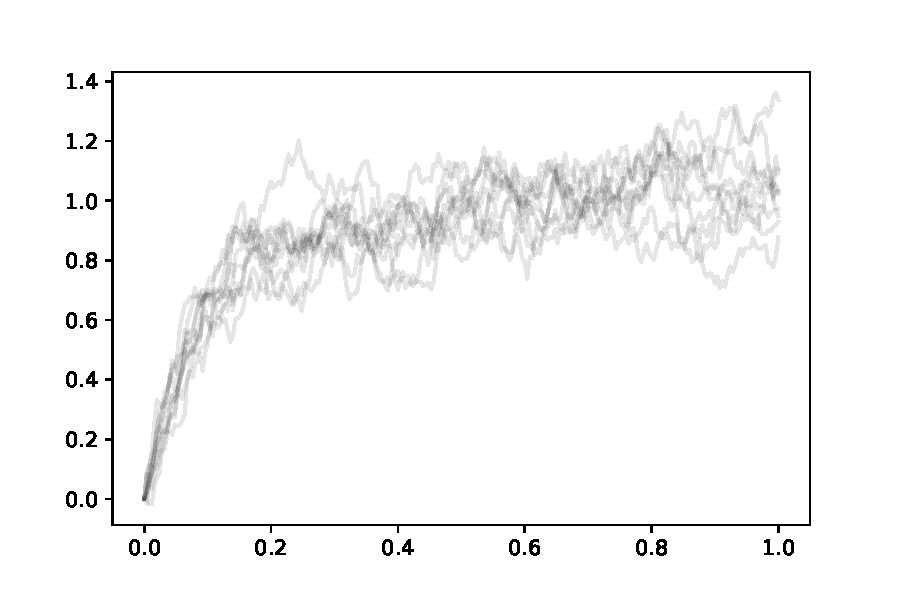
\includegraphics[width=\textwidth]{img/OU_em_10.pdf}
    \caption{10 trajectories of the OU equation with \( \theta = 10 \), \( \mu = 1 \), \( \sigma = 1/2 \) computed using the Euler--Maruyama method with a step size of \( \Delta t = 0.004 \).}
    \label{OU_em}
\end{subfigure}\hfill
\begin{subfigure}{.48\textwidth}\centering
    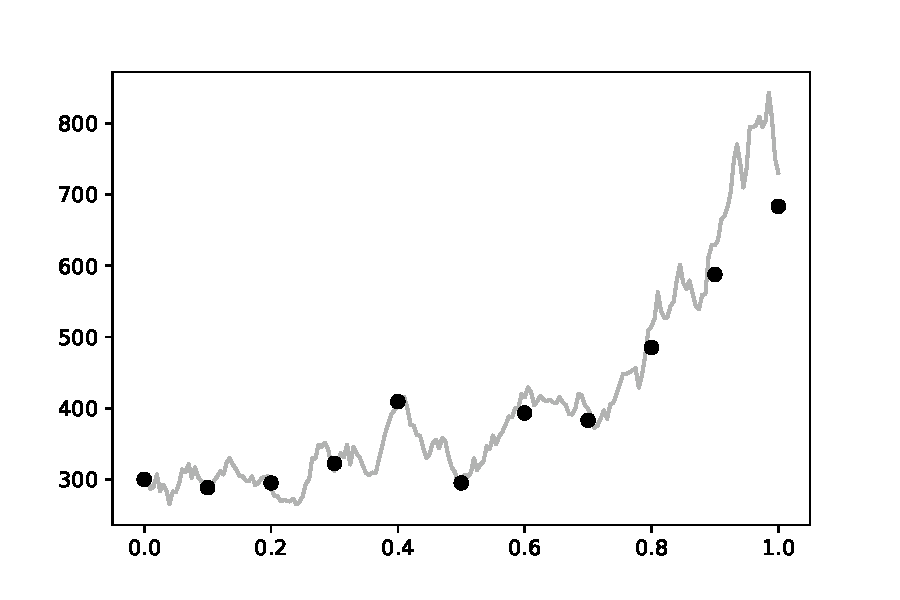
\includegraphics[width=\textwidth]{img/GBM_true_vs_10.pdf}
    \caption{Exact trajectory of Geometric Brownian motion with \( \mu = 1 \), \( \sigma = 1/2 \), and solution computed using the Euler--Maruyama method with a step size of \( \Delta t = 1/10 \).}
    \label{GBM_em}
\end{subfigure}
\caption{Basic numerical tests of Euler--Maruyama method}
\label{EM_tests}
\end{figure}


\section{Higher Order Methods}
The Euler--Maruyama method is commonly used due to its simplicity and ease of implementation. However, the strong convergence of this method is quite slow. As a result, higher order methods have been developed and studied. We introduce two methods in the hopes of illustrating how such methods can be derived. Both methods have strong and weak order one. A similar derivation can be found in \cite{holmes}.


By It\^o's Lemma (\ref{2dito}), if \( X_T \) is the solution to (\ref{intform}), for any sufficiently differentiable function \( f \) we have,
\begin{align}
    f(T,X_T) &= f(t,X_t) + \int_0^t \cM f(s,X_s)\d s + \int_0^t \cS f(s,X_s) \d W_s \label{ito1}
\end{align}
where,
\begin{align*}
    \cM := \pp{}{s} +  \mu(s,X_s)\pp{}{x} + \frac{1}{2}\sigma^2(s,X_s) \pp[2]{}{x}, && \cS := \sigma(s,X_s) \pp{}{x}
\end{align*}

Applying the relation in (\ref{ito1}) with \( f = \mu \) and \( f=\sigma \) gives,
\begin{align*}
    \mu(s,X_s) &= \mu(t,X_t) + \int_0^s \cM \mu(u,X_u) \d u + \int_0^s \cS \mu(u,X_u)\d W_u \\
    \sigma(s,X_s) &= \sigma(t,X_t) + \int_0^s \cM \sigma(u,X_u) \d u + \int_0^s \cS \sigma(u,X_u)\d W_u
\end{align*}

Therefore, inserting these expressions into (\ref{intform}) gives the relations,
\begin{align}
    X_t %&= X_t + \int_t^T \mu(t,X_t) \d s + \int_t^T \sigma(t,X_t) \d W_s + R \\
    &= X_0 + \mu(t,X_t) \int_0^t \d s +  \sigma(t,X_t)\int_0^t \d W_s + R \label{emexpr}
\end{align}
where
\begin{align}
    R &=  \int_0^t \int_0^s \cM \mu(u,X_u) \d u \d s + \int_0^t \int_0^s \cS \mu(u,X_u)\d W_u  \d s \tag*{}
    \\ &\hspace{4em} + \int_0^t \int_0^s \cM \sigma(u,X_u)\d u \d W_s + \int_0^t \int_0^s \cS \sigma(u,X_u) \d W_u \d W_s
\end{align}

Note the Euler--Maruyama method arises from (\ref{emexpr}) after dropping all the terms in \( R \) and setting \( T = t+\Delta t \).

Using the hueristics (\ref{heuristics}) the \( \d W_s \d W_t \) term is the highest order term of \( R \), so a higher order method must keep more of this term. We therefore apply the relation in (\ref{ito1}) with \( f = \cS \sigma \) to obtain,
\begin{align*}
    \cS \sigma(u,X_u) = \cS \sigma(t,X_t) + \int_{t}^{u} \cM \cM \sigma(v,X_v) \d v + \int_t^u \cS \cM \sigma(v,X_v) \d W_v
\end{align*}

Therefore,
\begin{align}
    X_t = X_0 + \int_0^t \mu(t,X_t) \d s + \int_0^t \sigma(t,X_t) \d W_s + \int_0^t \int_0^s \cS \sigma(t,X_t)  \d W_u \d W_v + R \label{milexpr}
\end{align}
where \( R \) contains higher order terms (and is different from the \( R \) in (\ref{emexpr})).


Applying It\^o's Lemma to \( f(x) = x^2 \) we obtained the well known result,
\begin{align*}
    \int_0^t \int_t^s \d W_u \d W_s
    = \int_0^t W_{s} \d W_s
    = \dfrac{1}{2} \left( (W_{t})^2 - t \right)
\end{align*}

Dropping all the terms in the new \( R \) and setting \( T = t+\Delta t \), (\ref{milexpr}) gives rise to the  Milstein method,
\begin{align*}
    \hat{X}_{t+\Delta t} &= \hat{X}_t + \mu(t,\hat{X}_{t}) \Delta t + \sigma(t,\hat{X}_{t}) \Delta W_{t} + \sigma(t,\hat{X}_t) \partial_x \sigma(t,\hat{X}_t) \left( (\Delta W_t)^2 - \Delta t \right)/2
\end{align*}

Both the Milstein and Forward Euler methods can be seen as Taylor series methods. Using similar approximations to what we have done here arbitrary order methods can be obtained. However, deriving and implementing such methods can easily become unwieldy. Therefore, as with deterministic IVP methods, the order of accuracy of a method must be balanced with the complexity of the method when deciding which method to apply.

As with deterministic IVP Taylor methods, knowing the derivative to a function is necessary. It is sometimes preferable to have methods which do not rely on knowing the derivative of any functions ahead of time.

We can approximate the \( x \)-derivative of \( \sigma \) by,
\begin{align}
    \pp{}{x}\sigma(\hat{X}_t,t) = \dfrac{\sigma(t,\hat{X}_t + \sigma(\hat{X})\sqrt{\Delta t}) - \sigma(t,\hat{X}_t)}{\sigma(\hat{X},t)\sqrt{\Delta t}} + \cO\left(\sigma(t,\hat{X}_t)\sqrt{\Delta t}\right) \label{derivapprox}
\end{align}

Using our heuristics (\ref{heuristics}) we expect substituting the right hand side to give a first order method which is the case (although not proved here).

Using the approximation in (\ref{derivapprox}) yields the strong first order Runge-Kutta method,
\begin{align*}
    \hat{X}_{t+\Delta t} &= \hat{X}_t + \mu(t,\hat{X}_{t}) \Delta t + \sigma(t,\hat{X}_{t}) \Delta W_{t} + \sigma(t,\hat{X}_t-X^*) \left( (\Delta W_t)^2 - \Delta t \right) / (2 \sqrt{\Delta t}) \\
    X^* &=  \hat{X}_t  + \sigma(t,\hat{X}_t)\sqrt{\Delta t}
\end{align*}

\section{Numerical Convergence Experiments}
In this section we conduct a few numerical experiments to see if they agree with the theoretical results presented above.

We implement the Euler-Maruyama and Runge-Kutta methods described above in Python using Numpy. These functions take in the Brownian motion in increment form as suggested previously. Note the notation change where we have denoted \( \mu \) and \( \sigma \) by \( a \) and \( b \).
\lstinputlisting[linerange=\#<start:em>-\#<end:em>]{solvers.py}
\lstinputlisting[linerange=\#<start:rk>-\#<end:rk>]{solvers.py}



Figure~\ref{weak_order_test} shows the absolute difference between the mean and variance of the actual solution and the mean and variance of various numerical methods. All three methods tested match the expected orders of weak convergence for the mean and variance of the process.

\begin{figure}[b!]\centering
\begin{subfigure}{.48\textwidth}\centering
    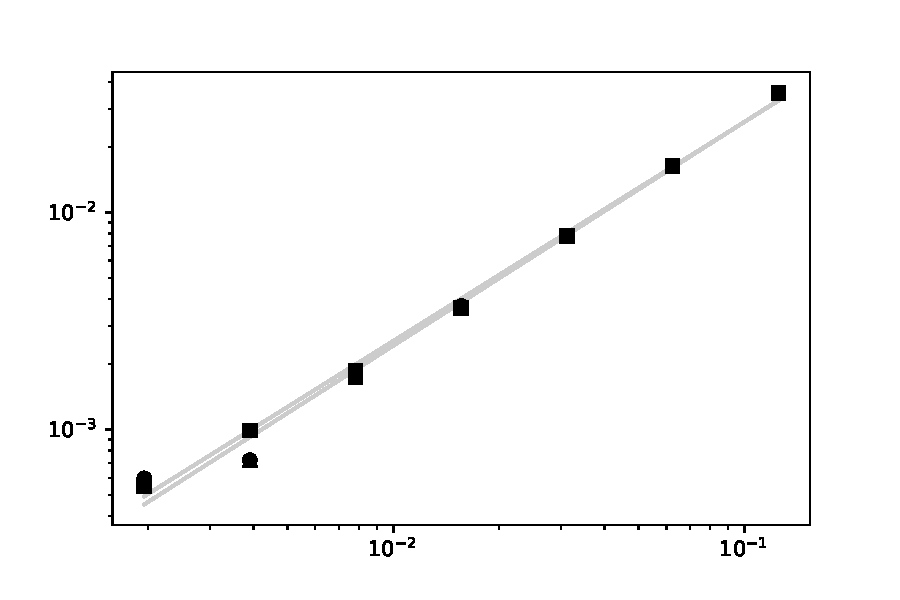
\includegraphics[width=\textwidth]{img/weak_order_2000.pdf}
    \caption{\( \dfrac{\big|\bE[X_T] - \bE[\hat{X}_T]\big|}{\big|\bE[X_T]\big|} \)}
    \label{mean}
\end{subfigure}
\begin{subfigure}{.48\textwidth}\centering
    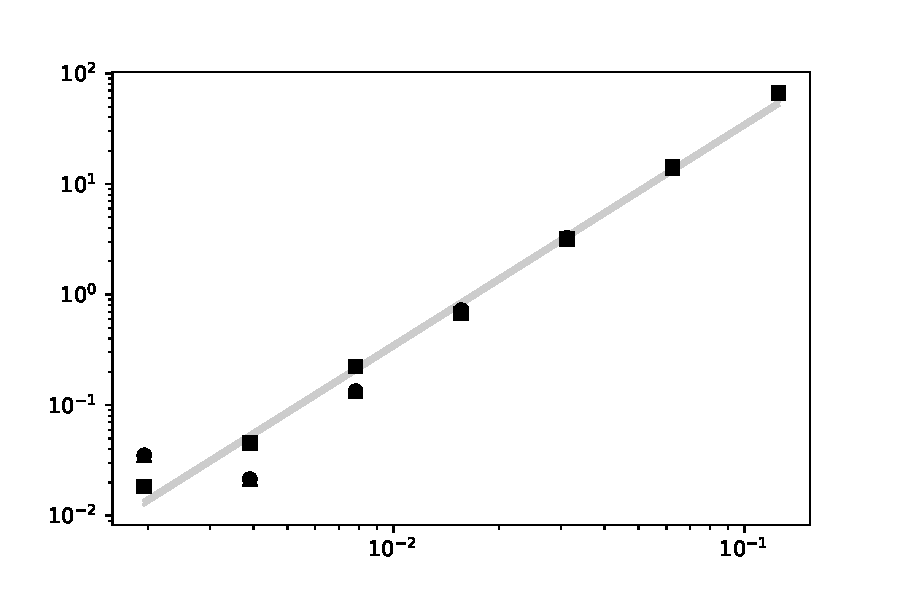
\includegraphics[width=\textwidth]{img/weak_order_2_mom_2000.pdf}
    \caption{\( \dfrac{\big|\bE[(X_T-\bE[X_T])^2] - \bE[(\hat{X}_T-\bE[X_T])^2]\big|}{\big|\bE[(X_T-\bE[X_T])^2]\big|} \) }
    \label{var}
\end{subfigure}
    \caption{Statistics based on 2000 trajectories, where \( T = 1 \) and \( X_t \) is a OU process with \( \theta = 1 \), \( \mu = 1 \), and \( \sigma = 1 \) for various \( \hat{X}_t \).  Circles correspond to the Euler--Maruyama method at various mesh sizes, triangles correspond to the Runge-Kutta method at various mesh sizes, and squares correspond to Euler--Maruyama method with \( \Delta W_t \in \{-\Delta t, \Delta t\} \). }
\label{weak_order_test}
\end{figure}

Note that the best fit lines in Figure~\ref{mean} have slopes of \protect\input{img/weak_order_em_2000.txt}\unskip, \protect\input{img/weak_order_rk_2000.txt}\unskip, and \protect\input{img/weak_order_em2_2000.txt}respectively. This is the expected weak convergence of order one.


Interestingly, the best fit lines in Figure~\ref{var} have slopes of \protect\input{img/weak_order_em_2_mom_2000.txt}\unskip, \protect\input{img/weak_order_rk_2_mom_2000.txt}\unskip, and \protect\input{img/weak_order_em2_2_mom_2000.txt}respectively. This seems to happen when adjusting the parameters of the processes as well as the number of trajectories used, etc. While it still satisfies the definition of weak convergence of order 1 it was unexpected.

We can now use our numerical solutions to generate trajectories of a Geometric Brownian motion. In particular, if for each trajectory we output the values of \( \Delta W_t \) at each time point, the Brownian motion \( W_t \) can be computer. This means we can compare our computed results at time \( T \) to the exact solution at time \( T \).

Figure~\ref{strong_order_test} shows the results of this for the Euler-Maruayma and Runge-Kutat methods. Note that the best fit lines have slopes of \protect\input{img/strong_order_em_1000.txt}and \protect\input{img/strong_order_rk_1000.txt}respectively. These are the order of strong convergence expected for both methods.

\begin{figure}[t!]\centering
    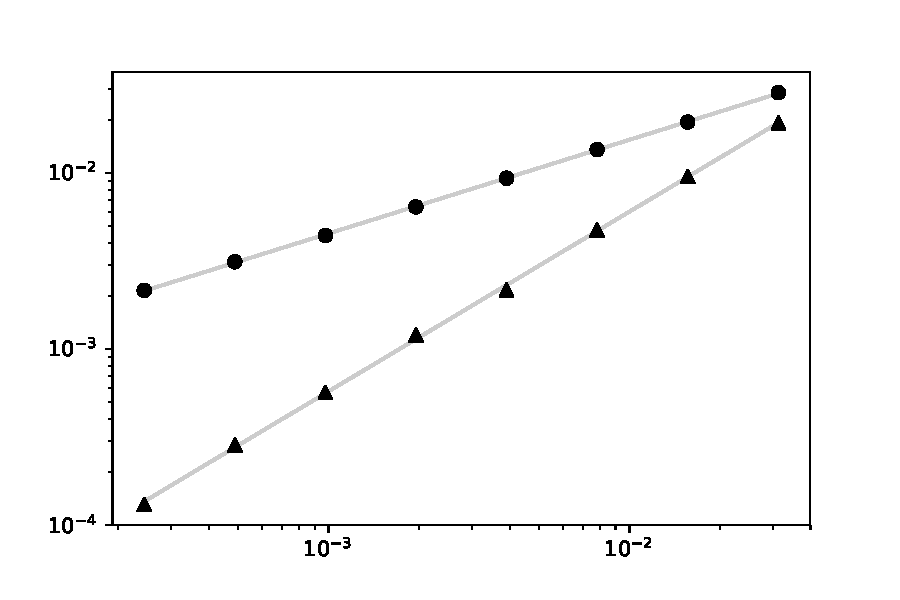
\includegraphics[width=.5\textwidth]{img/strong_order_1000.pdf}
    \caption{Values of \( \bE|X_T - \hat{X}_T|/\bE|X_T| \) approximated using 1000 trajectories, where \( T = 8 \) and \( X_t \) is a Geometric Brownian motion with \( \mu = 1 \) and \( \sigma = 1/2 \) for various \( \hat{X}_t \).  Circles correspond to the Euler--Maruyama method at various mesh sizes, and triangles correspond to the Runge-Kutta method at various mesh sizes.}
\label{strong_order_test}
\end{figure}

\section{Conclusion}
We introduce stochastic differential equations. In order to solve these numerically we introduced methods of generating Brownian motion on a discrete time mesh. We then introduced numerical SDE methods by approximating the solution using a (stochastic) Taylor expansion. Finally some numerical results were tested. For the most part the figures matched our expectations. However, the plot of Figure~\ref{var} shows that \( \big|\bE[(X_T-\bE[X_T])^2] - \bE[(\hat{X}_T-\bE[X_T])^2]\big|/\big|\bE[(X_T-\bE[X_T])^2]\big| \) goes to zero like \( k^2 \) rather than \( k \). At the moment it is not clear what affect the polynomial we chose, the processes, and the method have on this result. A more detailed look at this would be warranted.


\bibliography{project}{}
\bibliographystyle{ieeetr}

\pagebreak
\section{Code for Numerical Tests}
\lstinputlisting[basicstyle=\tiny\tt]{solvers.py}

\end{document}
